\documentclass[11pt]{article}
\usepackage{listings}
\usepackage{color}

\definecolor{dkgreen}{rgb}{0,0.6,0}
\definecolor{gray}{rgb}{0.5,0.5,0.5}
\definecolor{mauve}{rgb}{0.58,0,0.82}
\lstset{frame=tb,
  language=Java,
  aboveskip=3mm,
  belowskip=3mm,
  showstringspaces=false,
  columns=flexible,
  basicstyle={\small\ttfamily},
  numbers=none,
  numberstyle=\tiny\color{gray},
  keywordstyle=\color{blue},
  commentstyle=\color{dkgreen},
  stringstyle=\color{mauve},
  breaklines=true,
  breakatwhitespace=true,
  tabsize=3
}
%%%%%%%%%%%%%%%%%%%%% STYLE MACROS%%%%%%%%%%%%%%%%%%%%


% Page format commands

\setlength{\parindent}{0in}    
\setlength{\parskip}{0.5\baselineskip}

\hoffset        = -1.0 in
\voffset        = -1.0 in

% US letter
%\paperheight    = 11.0 in
%\paperwidth     =  8.5 in

% A4
\paperheight    = 297 mm
\paperwidth     = 210 mm


\topmargin      = 1.0 in
\headheight     = \baselineskip
\headsep        = \baselineskip
\footskip       = 0.5 in
\textheight     = \paperheight
\addtolength{\textheight}{-\topmargin}
\addtolength{\textheight}{-\headheight}
\addtolength{\textheight}{-\headsep}
\addtolength{\textheight}{-\footskip}
\addtolength{\textheight}{-0.5in}   % space after page number at bottom

\textwidth      = \paperwidth
\oddsidemargin  = 1.0 in
\evensidemargin = 1.0 in
\addtolength{\textwidth}{-\oddsidemargin}
\addtolength{\textwidth}{-\evensidemargin}

\linewidth      = \textwidth

\usepackage{listings}
\usepackage{color}
\usepackage{subfig}
\usepackage{float}

\lstset{frame=tb,
  aboveskip=3mm,
  belowskip=3mm,
  showstringspaces=false,
  columns=flexible,
  basicstyle={\small\ttfamily},
  numbers=left,
  stringstyle=\color{mauve},
  breaklines=true,
  breakatwhitespace=true
  tabsize=3
}



%%%%%%%%%%%%%%%%%%%%%%%%%% PACKAGES %%%%%%%%%%%%%%%%%%%%%%%%%%%%%%%%%%
%\documentclass[a4paper,twoside,english]{amsart}
\usepackage{amsfonts,amsthm,amsmath,amssymb,latexsym,comment}

%\usepackage[T1]{fontenc}
%\usepackage[latin1]{inputenc}
\usepackage{setspace}
\usepackage{verbatim}
\usepackage{color}
%\usepackage{algorithmic}
%\usepackage{algorithm}
\usepackage{xspace}
\usepackage{graphics}
%\usepackage{floatflt}
%\usepackage{wrapfig}
\usepackage{url,cite}

%%% SIMONS PACKAGES
%\usepackage{graphicx,color}
%\usepackage{amsmath,amscd}
% \usepackage{enumitem}
% \usepackage{wrapfig}
% \usepackage{subfigure}
% \usepackage{picins}
 \usepackage{tikz}
 \usetikzlibrary{shapes,arrows}









%%%%%%%%%%%%%%%%%%%%%%% IDENTIFIER MACROS %%%%%%%%%%%%%%%%%%%%%%%%%%%
\newcommand{\IDENT}[1]{\ensuremath{\mathit{#1}}}
\newcommand{\EMTH}[1]{\ensuremath{#1}\xspace}


\newcommand{\spc}{\ensuremath{\eta}}           % specification formula
\newcommand{\spcb}{\ensuremath{\eta_B}}      % box specification formula
\newcommand{\cfm}{\ensuremath{\vphi}}         % coupling formula
\newcommand{\MA}{\ensuremath{M_A}}            % abstract structure 
%\newcommand{\BA}{\ensuremath{B_A}\xspace}              % abstract box 
\newcommand{\BA}{\EMTH{\IDENT{B}_A}}
%\newcommand{\BA}{\IDENT{B_A}}
\newcommand{\BD}{\ensuremath{\widehat{B}}\xspace}         % dreived box 
\newcommand{\BM}{\ensuremath{B_M}\xspace}          % situated box
\newcommand{\preB}{\ensuremath{pre_B}\xspace}      % interface state for box
\newcommand{\postB}{\ensuremath{post_B}\xspace}
\newcommand{\inB}{\EMTH{\IDENT{in}_B}}
\newcommand{\stB}{\EMTH{\IDENT{start}_B}}
\newcommand{\intB}{\EMTH{\IDENT{int}_B}}
\newcommand{\rexB}{\EMTH{\IDENT{O}_B^r}}   % reachable exit states of B
\newcommand{\exB}{\EMTH{\IDENT{O}_B}}   % exit states of B

\newcommand{\mscc}{\EMTH{\IDENT{C}}}   % mscc collapse of M
\newcommand{\BN}{\ensuremath{\widehat{B}}\xspace}         % B           collapsed to a single node

\newcommand{\APB}{\EMTH{\IDENT{\AP}_B}}   % atomic props of B
\newcommand{\APC}{\EMTH{\IDENT{\AP}_C}}   % atomic props of coupling formula 
\newcommand{\APS}{\EMTH{\IDENT{\AP}_\spc}}   % atomic props of spec formula 
\newcommand{\APF}{\EMTH{\IDENT{\AP''}}}   % atomic props in weak forward sim definition




%%%%%%%%%%%%%%%%%%%%%%% FROM MOUHAMMADS THESIS %%%%%%%%%%%%%%%%%%%%%%%%%%%

\newcommand{\evpa}{\ensuremath{\equiv_{p,a}}}
\newcommand{\evpna}{\ensuremath{\equiv_{p}}}
\newcommand{\evsa}{\ensuremath{\equiv_{s,a}}}
\newcommand{\evsna}{\ensuremath{\equiv_{s,p}}}

\newcommand{\eqc}[1]{\ensuremath{[#1]}}

\newcommand{\stt}{~|~}

\newcommand{\AS}{\mathit{AS}}
\newcommand{\SUB}{\mathit{SUB}}

\newcommand{\ovl}{\overline}



%%%%%%%%%%%%%%%%%%%%%%%%%%% REPAIR SPECIFIC MACROS %%%%%%%%%%%%%%%%%%%%%%%%%%%%

\newcommand{\Eshmun}{\textsf{Eshmun}\xspace}

\newcommand{\tool}[1]{\texttt{#1}}
\newcommand{\st}[1]{\tool{#1}}


\newcommand{\rprob}[2]{\ensuremath{\tpl{#1,#2}}}   %repair problem: rprob{M}{\eta}

\newcommand{\rfor}[2]{\ensuremath{\mathit{repair(#1,#2)}}}   %repair formula: rfor{M}{\eta}
\newcommand{\repfor}{\ensuremath{\mathit{repair}}}

\newcommand{\rmod}[2]{\ensuremath{\mathit{model(#1,#2)}}}    % repaired model: rmod{M}{\Val}
\newcommand{\repmod}{\ensuremath{\mathit{model}}}

\newcommand{\lab}[1]{\ensuremath{\mathcal L}(#1)}
\newcommand{\new}[1]{\ensuremath{\mathit{new}(#1)}}
\newcommand{\old}[1]{\ensuremath{\mathit{old}(#1)}}

\newcommand{\kdef}{\ensuremath{(S_0, S, R, L, \AP)}\xspace}
\newcommand{\kripkedef}{\ensuremath{(S_0, S, R, L, \AP)}\xspace}

\newcommand{\kdefp}{\ensuremath{(S'_0, S', R', L', \AP)}\xspace}
\newcommand{\kripkeprimedef}{\ensuremath{(S'_0, S', R',L',\AP)}\xspace}

\newcommand{\kdefpp}{\ensuremath{(S''_0, S'', R'', L'', \AP)}\xspace}

\newcommand{\rkdef}{\ensuremath{(S_0, S, R, L, \AP)}\xspace} % repaired kripke
\newcommand{\qkdef}{\ensuremath{(\ovl{S}_0, \ovl{S}, \ovl{R}, \ovl{L},\AP)}\xspace} % quotient kripke def
\newcommand{\akdef}{\ensuremath{(\ovl{S}_0, \ovl{S}, \ovl{R}, \ovl{L},\APS)}\xspace} % abstract kripke def

\newcommand{\qM}{\ensuremath{\ovl{M}}\xspace} % quotient kripke
\newcommand{\aM}{\ensuremath{\ovl{M}}\xspace} % abstract kripke 
\newcommand{\rM}{\ensuremath{M'}\xspace} % repaired kripke 





\newcommand{\prkdef}[1]{\ensuremath{(S_0^{#1}, S_{#1}, R_{#1}, L_{#1}, \AP_{#1})}\xspace} % pair kripke

\newcommand{\FL}{\ensuremath{\mathit{sub}}}
\newcommand{\cgsdef}{\ensuremath{(s_0, S, R, L,\sigma)}\xspace}

\newcommand{\Val}{\mathcal{V}}



\newcommand{\fsim}{\le}

\newcommand{\lfsim}[1]{\le_{#1}}





%%%%%%%%%%%%%%%%%%%% PHONE CALL EXAMPLE%%%%%%%%%%%%%%%%%%%%%%%%%5
\newcommand{\LBL}[1]{\mathit{#1}}

\newcommand{\snd}{\LBL{snd}}
\newcommand{\wt}{\LBL{wt}}
\newcommand{\tmt}{\LBL{tmt}}
\newcommand{\nk}{\LBL{nk}}
\newcommand{\ack}{\LBL{ack}}

\newcommand{\ok}{\LBL{ok}}
\newcommand{\fl}{\LBL{fl}}

\newcommand{\suc}{\LBL{sc}}
\newcommand{\ab}{\LBL{ab}}



%%%%%%%%%%%%%%%%%%%% BARRIER SYNC EXAMPLE %%%%%%%%%%%%%%%%%%%%%%%%%%%%%%%%%%%%

\newcommand{\SA}{\LBL{sa}}
\newcommand{\EA}{\LBL{ea}}
\newcommand{\SB}{\LBL{sb}}
\newcommand{\EB}{\LBL{eb}}




%%%%%%%%%%%%%%%%%%%%%%%%%%%%%%% MISC %%%%%%%%%%%%%%%%%%%%%%%%%%%%%%%%%%%%%%%
 
\newcommand{\pkg}[1]{\texttt{#1}\xspace}


\newcommand{\cmnt}{\ensuremath{\rhd}}
\newcommand{\case}[1]{\ul{\textit{#1}}}

\newcommand{\ie}{i.e.,\xspace}
\newcommand{\eg}{e.g.,\xspace}
\newcommand{\wrt}{w.r.t.\xspace}
\newcommand{\etal}{et.~al.\xspace}


\newcommand{\remove}[1]{}

\newcommand{\KS}{Kripke strucuture\xspace}

%%%%%%%%%%%%%%%%%%%%%%%%%%%%%% ABBREVIATIONS %%%%%%%%%%%%%%%%%%%%%%%%%%%%%%%

%% Lists
\newcommand{\be}{\begin{itemize}}
\newcommand{\ee}{\end{itemize}}
\newcommand{\bn}{\begin{enumerate}}
\newcommand{\en}{\end{enumerate}}


%% Theorem-like Environments
\newcommand{\bp}{\begin{proposition}}
\newcommand{\ep}{\end{proposition}}
\newcommand{\bl}{\begin{lemma}}
\newcommand{\el}{\end{lemma}}
\newcommand{\bco}{\begin{corollary}}
\newcommand{\eco}{\end{corollary}}
\newcommand{\bt}{\begin{theorem}}
\newcommand{\et}{\end{theorem}}
\newcommand{\bpr}{\begin{proof}}
\newcommand{\epr}{\end{proof}}
\newcommand{\bd}{\begin{definition}}
\newcommand{\ed}{\end{definition}}


%% Equation Environments
\newcommand{\beqn}{\begin{centeqn}}
\newcommand{\eeqn}{\end{centeqn}}
\newcommand{\beqnnbsp}{\begin{centeqn-nbsp}}
\newcommand{\eeqnnbsp}{\end{centeqn-nbsp}}
\newcommand{\bleqn}[1]{\begin{centlabeqn}{#1}}
\newcommand{\eleqn}{\end{centlabeqn}}
\newcommand{\bleqnnbsp}[1]{\begin{centlabeqn-nbsp}{#1}}
\newcommand{\eleqnnbsp}{\end{centlabeqn-nbsp}}

%% Misc
\newcommand{\bc}{\begin{center}}
\newcommand{\ec}{\end{center}}
\newcommand{\ul}{\underline}
\newcommand{\bs}{\bigskip}
\newcommand{\ms}{\medskip}
\renewcommand{\ss}{\smallskip}

\newcommand{\bfg}{\begin{figure}}
\newcommand{\efg}{\end{figure}}








%%%%%%%%%%%%%%%%%%%%%%%%% EQUATION ENVIRONMENTS %%%%%%%%%%%%%%%%%%%%%%%%%%%%%%%%

\newenvironment{centeqn}	% centered equation environment
   {{\ss\\ \hspace*{\fill}}} 
   {\hspace*{\fill}\ss\\}

\newsavebox{\EqnLabel}
\newenvironment{centlabeqn}[1]		% centered labeled equation environment
   {\sbox{\EqnLabel}{#1}
    {\\ \hspace*{\fill}}
   } 
   {\hfill{\makebox[0in][r]{\usebox{\EqnLabel}}}\ms\\}

\newenvironment{centeqn-nbsp} % centered equation - no vertical space at the bottom
   {{\ms\\ \hspace*{\fill}}}
   {\hspace*{\fill}}



%%%%%%%%%%%%%%%%%%%% FORMATTING COMMANDS %%%%%%%%%%%%%%%%%%%%%%%%%%%

\newcommand{\intrdef}{\emph}	
\newcommand{\intr}{\emph}	
\newcommand{\empi}{\textit}	
\newcommand{\empb}{\textbf}	
				




%%%%%%%%%%%%%%%%%%%%%%% GENERAL MATH SYMBOLS %%%%%%%%%%%%%%%%%%%%%%%%%%%%%%

\newcommand{\setIns}[2]{\ensuremath{ #1 \gt #1 \un #2 }}
\newcommand{\setInsS}[2]{\ensuremath{ #1 \gt #1 \un \set{#2} }}
\newcommand{\setDel}[2]{\ensuremath{ #1 \gt #1 - #2 }}
\newcommand{\setDelS}[2]{\ensuremath{ #1 \gt #1 - \set{#2} }}


\newcommand{\mucalc}{{\ensuremath{\mu}-calculus }}
\newcommand{\ttt}{\mathit{tt}}
\newcommand{\fff}{\mathit{ff}}
\renewcommand{\tt}{\ensuremath{\mathit{tt}}}     % semantic true and false
\newcommand{\ff}{\ensuremath{\mathit{ff}}}


\newcommand{\ATLA}{\ll\!A\!\gg}
\newcommand{\ATLAneg}{\ll\!\Sigma - A\!\gg}
\newcommand{\Gg}{{\mathcal{G} }}
\newcommand{\vphi}{\varphi}


\newcommand{\ba}{\bigwedge}	
\newcommand{\AND}{\bigwedge}
\newcommand{\INT}{\bigcap}
\newcommand{\bo}{\bigvee}	
\newcommand{\OR}{\bigvee}
\newcommand{\UN}{\bigcup}
\newcommand{\PA}{/\!/}		% parallel assignment

\newcommand{\oneton}{\{1, \ldots, n\}}
\newcommand{\rng}[2]{\{#1, \ldots, #2\}}

\newcommand{\ar}{\rightarrow}	% abbreviated rightarrow
\newcommand{\cat}{\frown}
\newcommand{\choice}{\mbox{$[\hspace*{-1.0pt}]$}}
\renewcommand{\d}{\, : \,}	% separator in quantified formulae
\newcommand{\df}{\mbox{$\:\stackrel{\rm df}{=\!\!=}\:$}}
\newcommand{\ev}{\equiv}
\newcommand{\ex}{\exists}
\newcommand{\fa}{\forall}
\newcommand{\halfind}{\hspace*{1.5em}}
\newcommand{\ifof}{\Longleftrightarrow}	
%\newcommand{\iff}{\Leftrightarrow}	
\newcommand{\imp}{\Rightarrow}		
%\newcommand{\implies}{\imp}		
\newcommand{\ind}{\hspace*{3.0em}}
\newcommand{\ints}{\cap}
\renewcommand{\l}{\ell}
\newcommand{\la}[1]{\mbox{$\, \stackrel{#1}{\rightarrow} \,$}}

\newcommand{\lra}{\mbox{$\longrightarrow$}}

\newcommand{\mstr}[1]{\ensuremath{`` #1 \mbox{''} }}       % string in math mode

\newcommand{\pind}{\hspace*{3.0em}}
\newcommand{\pl}{\!\parallel\!}
\newcommand{\pj}{\ensuremath{\upharpoonright}}
\newcommand{\s}{\mbox{$\hspace{-1pt}-\hspace{-2pt}$}}
\newcommand{\sat}{\models}
\newcommand{\set}[1]{\ensuremath{\{#1\}}}
\newcommand{\tpl}[1]{\ensuremath{\langle#1\rangle}}


%\newcommand{\spc}{\mbox{\vspace{-0.25in}}}
%%\newcommand{\st}[2]{\mbox{$\stackrel{#1}{#2}$}}	% abbreviated stackrel
\newcommand{\sub}{\subseteq}
\newcommand{\tl}[1]{\mbox{$\tilde{#1}$}}% abbreviated tilde
\newcommand{\un}{\cup}
\newcommand{\up}{\mbox{$\hspace{-0.1em}\uparrow\hspace{-0.1em}$}}
\newcommand{\dn}{\mbox{$\hspace{-0.1em}\downarrow\hspace{-0.1em}$}}

\newcommand{\struct}[2]{\raisebox{-0.1in}{$\stackrel { \displaystyle
#1} {\scriptstyle #2}\,$}}





%%%%%%%%%%%%%%%%%%%%%%%%%%% LIST ENVIRONMENTS %%%%%%%%%%%%%%%%%%%%%%%%%%%%%%%

\newenvironment{lst}{\begin{list}	
                       {}
                       {\setlength{\topsep}{0em}
                        \setlength{\itemsep}{0em}
			\setlength{\leftmargin}{0.5in}
		     }}
                    {\end{list}}

\newenvironment{blst}{\begin{list}		% bullet list
                       {--}
                       {\setlength{\topsep}{0em}
                        \setlength{\itemsep}{0em}
			\setlength{\leftmargin}{0.25in}
		     }}
                    {\end{list}}

\newcounter{levelone}
\newenvironment{nlst1}{\begin{list}	% 1'st level enumerated list
                       {\arabic{levelone}.}
                       {\usecounter{levelone}
			\setlength{\topsep}{0em}
                        \setlength{\itemsep}{0em}
			\setlength{\leftmargin}{0.25in}
		     }}
                    {\end{list}}


\newcounter{leveltwo}
\newenvironment{nlst2}{\begin{list}	% 2'nd level enumerated list
                       {(\alph{leveltwo})}
                       {\usecounter{leveltwo}
			\setlength{\topsep}{0em}
                        \setlength{\itemsep}{0em}
			\setlength{\leftmargin}{0.4in}
		     }}
                    {\end{list}}




%%%%%%%%%%%%%%%%%%%%%%%%%%%%%%%%% MISC  %%%%%%%%%%%%%%%%%%%%%%%%%%%%%%%

%\renewcommand{\S}{{\cal S}}
\newcommand{\Fa}{\ensuremath{\mathcal F}\xspace}


%%%%%%%%%%%%%%%%%%%%%%%%%%% MISC ENVIRONMENTS %%%%%%%%%%%%%%%%%%%%%%%%%%%%%%%

% \newenvironment{proof}{\vspace{-1.0ex}\textit{Proof.} }		% Proof environment
%                       {\hfill{$\Box$}}







% \newcommand{\stof}[1]{\{\hspace*{-0.3em}|#1|\hspace*{-0.3em}\}}
% 				 % state to formula conversion
% 				 % for local states (intended
% 				 % to replace \F above


% \newcommand{\qf}[3]{#1 #2 \d ( #3 )}   %% quatified formula --
% 				       %% currently unused


% \newcommand{\CL}{\mathit{CL}}



%%% SIMONS REFERENCES MACROS

\newcommand{\defn}[1]{Def.~\ref{defn:#1}}
\newcommand{\sfig}[1]{Figure~\ref{fig:#1}}    %start of sentence
\newcommand{\fig}[1]{Fig.~\ref{fig:#1}}
\newcommand{\tab}[1]{Tab.~\ref{tab:#1}}
\newcommand{\eq}[1]{(\ref{eq:#1})}
\newcommand{\res}[1]{(\ref{res:#1})}
\newcommand{\secn}[1]{Sect.~\ref{secn:#1}}
\newcommand{\rem}[1]{Rem.~\ref{rem:#1}}
\newcommand{\ntn}[1]{Not.~\ref{ntn:#1}}
\newcommand{\lem}[1]{Lem.~\ref{lem:#1}}
\newcommand{\cor}[1]{Cor.~\ref{cor:#1}}
\newcommand{\thm}[1]{Th.~\ref{thm:#1}}
\newcommand{\app}[1]{App.~\ref{app:#1}}
\newcommand{\axs}[1]{Ax.~\ref{ax:#1}}
\newcommand{\axss}[2]{Ax.~\ref{ax:#1}, \ref{ax:#2}}
\newcommand{\ax}[1]{Ax.~\ref{ax:#1}}
\newcommand{\prop}[1]{Prop.~\ref{prop:#1}}
\newcommand{\clause}[1]{Clause~\ref{clause:#1}}



%%%%%%%%%%%%%%% TEMPORAL LOGIC SYMBOLS --- CTL* and CTL %%%%%%%%%%%%%%%%%%%
\newcommand{\TLM}[1]{\ensuremath{\mathsf{#1}}}   % TLM = temporal logic modality

\newcommand{\yld}{\ensuremath{\vdash_{CTL}}}
\newcommand{\satCTL}{\ensuremath{\models}}
\newcommand{\satf}{\models_{\f}}
\newcommand{\AP}{\ensuremath{\mathit{AP}}\xspace}
\newcommand{\ACTL}{\ensuremath{\mathrm{ACTL}}\xspace}  
\newcommand{\ACTLm}{\mbox{$\mathrm{ACTL}^-$}}  
\newcommand{\ACTLS}{\mbox{$\mathrm{ACTL}^*$}}  
\newcommand{\ATL}{\ensuremath{\mathrm{ATL}}\xspace}  
\newcommand{\CTL}{\ensuremath{\mathrm{CTL}}\xspace}  
\newcommand{\CTLS}{\ensuremath{\mathrm{CTL}^*}\xspace}
\newcommand{\SH}{\mbox{$\cal SH$}}  

\newcommand{\A}{\TLM{A}}
\newcommand{\E}{\TLM{E}}
\newcommand{\F}{\TLM{F}}
\newcommand{\G}{\TLM{G}}
\newcommand{\U}{\TLM{U}}
\newcommand{\Uw}{\TLM{Uw}}
\newcommand{\V}{\TLM{V}}
\newcommand{\W}{\TLM{W}}
\newcommand{\X}{\TLM{X}}
\newcommand{\Y}{\TLM{Y}}

\newcommand{\true}{\ensuremath{\mathsf{true}}\xspace}
\newcommand{\false}{\ensuremath{\mathsf{false}}\xspace}

\newcommand{\AG}{\TLM{AG}}
\newcommand{\EG}{\TLM{EG}}
\newcommand{\AF}{\TLM{AF}}
\newcommand{\EF}{\TLM{EF}}
\newcommand{\AU}{\TLM{AU}}
\newcommand{\EU}{\TLM{EU}}
\newcommand{\AV}{\TLM{AV}}
\newcommand{\EV}{\TLM{EV}}
\newcommand{\AX}{\TLM{AX}}
\newcommand{\EX}{\TLM{EX}}



%\newcommand{\ea}{\raisebox{0.2ex}{$\stackrel{\infty}{\textsf{G}}$}}  %10ptfont
%\newcommand{\ea}{\raisebox{0.22ex}{$\stackrel{\infty}{\textsf{G}}$}}
\newcommand{\ea}{\raisebox{0ex}{$\stackrel{\infty}{\textup{\textsf{G}}}$}}

%\newcommand{\io}{\raisebox{0.2ex}{$\stackrel{\infty}{\textup{\textsf{F}}}$} %10ptfont
%\newcommand{\io}{\raisebox{0.22ex}{$\stackrel{\infty}{\textsf{F}}$}}
\newcommand{\io}{\raisebox{0ex}{$\stackrel{\infty}{\textup{\textsf{F}}}$}}




%%%%%%%%%%%%%%%%%%%% THEOREM-LIKE ENVIRONMENT DECLARATIONS %%%%%%%%%%%%%%%%%%%

\newtheorem{theorem}{Theorem}
\newtheorem{conjecture}{Conjecture}
\newtheorem{lemma}{Lemma}
\newtheorem{proposition}[lemma]{Proposition}
\newtheorem{definition}{Definition}
\newtheorem{example}{Example}
\newtheorem{claim}{Claim}
\newtheorem{corollary}{Corollary}
\newtheorem{introtheorem}{Theorem}
\newtheorem{assumption}{Assumption}



\remove{

\newtheorem{theorem}{Theorem}
\newtheorem{lemma}[theorem]{Lemma}
\newtheorem{proposition}[theorem]{Proposition}
\newtheorem{corollary}[theorem]{Corollary}

\newtheorem{definition}{Definition}

\newtheorem{subtheorem}{Theorem}[subsection]
\newtheorem{sublemma}[subtheorem]{Lemma}
\newtheorem{subproposition}[subtheorem]{Proposition}
\newtheorem{subcorollary}[subtheorem]{Corollary}

\newtheorem{subdefinition}[subtheorem]{Definition}


\newtheorem{observation}{Observation}

%%%\newdef{example}{Example}  % CURRENTLY UNUSED
}



%%%%%%%%%%%%%%%%%%%%%%%%%%%% COMPLEXITY THEORY %%%%%%%%%%%%%%%%%%%%%%%%%%

\newcommand{\ELTIME}{\textsc{Elementary}\xspace}
\newcommand{\DTIME}[1]{\ensuremath{\mathrm{DTime(}#1\mathrm{)}}}
\newcommand{\NTIME}[1]{\ensuremath{\mathrm{NTime(}#1\mathrm{)}}}
\newcommand{\DSPACE}[1]{\ensuremath{\mathrm{DSpace(}#1\mathrm{)}}}
\newcommand{\ExpTime}{\textsc{ExpTime}\xspace}
\newcommand{\EXPTIME}[1]{\ensuremath{#1}\ExpTime}
\newcommand{\EXPSPACE}[1]{\ensuremath{{#1}\mathrm{ExpSpace}}}
\newcommand{\ATIME}[1]{\ensuremath{\mathrm{ATime(}#1\mathrm{)}}}
\newcommand{\ASPACE}[1]{\ensuremath{\mathrm{ASpace(}#1\mathrm{)}}}
\newcommand{\AEXPTIME}[1]{\ensuremath{{#1}\mathrm{AExpTime}}}
\newcommand{\AEXPSPACE}[1]{\ensuremath{{#1}\mathrm{AExpSpace}}}
\newcommand{\tSAT}{\ensuremath{\mathrm{3SAT}}\xspace}
\newcommand{\tcnf}{\ensuremath{\mathrm{3cnf}}\xspace}





\def\rien{\rule{0pt}{0pt}}
\newcommand\NEG{\mathop{\;\;\mathrm{NEG}\;}}

% unused
%\newcommand*{\pcgsdef}{\ensuremath{(S, \{s_{0}\},  R,L,P,\sigma)}}
\newcommand*{\markovdef}{\ensuremath{(S, \{s_{0}\},  R,L,P)}}
\newcommand{\refuter}{\ensuremath{\forall}belard\xspace}
\newcommand{\verifier}{\ensuremath{\exists}loise\xspace}
\def\seqcalcZ#1{\begin{array}{@{}c@{}}\rien\vspace{-15pt}\\\displaystyle\frac{}{#1}\vspace{-17pt}\\\rien\end{array}}
\def\seqcalc#1#2{\begin{array}{@{}c@{}}\rien\vspace{-15pt}\\\displaystyle\frac{#1}{#2}\vspace{-17pt}\\\rien\end{array}}
\def\seqcalcT#1#2#3{\begin{array}{@{}c@{}}\rien\vspace{-15pt}\\\displaystyle\frac{#1\qquad#2}{#3}\vspace{-17pt}\\\rien\end{array}}


\newcommand{\pc}[1]{{#1}}    %% font for pseudocode
%\newcommand{\pc}[1]{\codetext{#1}}    %% font for pseudocode

%%%%%%%%%%%%%% MACROS FOR NUMBERED LINES IN CODE TABBING ENVIRONMENT %%%%%%%%%%%%%%%%

\newcounter{lctr}

\newcommand{\li}{\addtocounter{lctr}{1}\arabic{lctr}.}
\newcommand{\lio}[1]{\addtocounter{lctr}{1}\arabic{lctr}.\>\ensuremath{#1}\\}
\newcommand{\lit}[1]{\addtocounter{lctr}{1}\arabic{lctr}.\>\>\ensuremath{#1}\\}
\newcommand{\lih}[1]{\addtocounter{lctr}{1}\arabic{lctr}.\>\>\>\ensuremath{#1}\\}

%%%% 2'nd argument is for a commment
\newcommand{\lioc}[2]{\addtocounter{lctr}{1}\arabic{lctr}.\>\ensuremath{#1}\`{#2}\\}
\newcommand{\litc}[2]{\addtocounter{lctr}{1}\arabic{lctr}.\>\>\ensuremath{#1}\`{#2}\\}
\newcommand{\lihc}[2]{\addtocounter{lctr}{1}\arabic{lctr}.\>\>\>\ensuremath{#1}\`{#2}\\}




%%%%%%%%%%%%%%%%%%%%%%%%%%% PSEUDOCODE SECTION

\newcommand{\gt}{\ensuremath{:=}}   % assignment
\newcommand{\swap}{\ensuremath{\leftrightarrow}}   % swap two vars

\newcommand{\pseudocode}[1]{\ensuremath{\mathbf{#1}\ }}
\newcommand{\pseudocodensp}[1]{\ensuremath{\mathbf{#1}}}
%\newcommand{\pseudocode}[1]{\mbox{${\bf #1}$}\xspace}

\newcommand{\IFC}[1]{\pseudocode{if}\ (\ensuremath{#1})}
\newcommand{\WHILEC}[1]{\pseudocode{while}\ (\ensuremath{#1})}
\newcommand{\RETURNE}[1]{\pseudocodensp{return}(\ensuremath{#1})}

\newcommand{\CASE}{\pseudocode{case}}
\newcommand{\ENDCASE}{\pseudocode{endcase}}
\newcommand{\IF}{\pseudocode{if}}
\newcommand{\WHILE}{\pseudocode{while}}
\newcommand{\FOR}{\pseudocode{for}}
\newcommand{\FORALL}{\pseudocode{forall}}
\newcommand{\FI}{\pseudocode{fi}}
\newcommand{\THEN}{\pseudocode{then}}
\newcommand{\ELSE}{\pseudocode{else}}
\newcommand{\ELSF}{\pseudocode{else\ if}}
\newcommand{\ENDIF}{\pseudocode{endif}}
\newcommand{\ENDFOR}{\pseudocode{endfor}}
\newcommand{\DO}{\pseudocode{do}}
\newcommand{\OD}{\pseudocode{od}}
\newcommand{\ENDWHILE}{\pseudocode{endwhile}}
\newcommand{\BEGIN}{\pseudocode{begin}}
\newcommand{\END}{\pseudocode{end}}
\newcommand{\PROC}{\pseudocode{procedure}}
\newcommand{\CALL}{\pseudocode{call}}
\newcommand{\VAL}{\pseudocode{value}}
\newcommand{\VALRES}{\pseudocode{value\!-\!result}}
\newcommand{\RES}{\pseudocode{result}}
\newcommand{\RETURN}{\pseudocode{return}}
\newcommand{\REPEAT}{\pseudocode{repeat}}
\newcommand{\DOWNTO}{\pseudocode{downto}}
\newcommand{\TO}{\pseudocode{to}}

\newcommand{\function}{\pseudocode{function}}
\newcommand{\operation}{\pseudocode{operation}}

\newcommand{\newo}{\pseudocode{new}}
\renewcommand{\int}{\pseudocode{int}}



%% Algorithm names

\newcommand{\ANAME}[1]{\ensuremath{\mathsf{#1}}}

\newcommand{\compRepFor}{\ANAME{ComputeRepairFormula}}
\newcommand{\compRepForA}[1]{\ANAME{ComputeRepairFormula}(#1)}

\newcommand{\initRepFor}{\ANAME{InitializeRepairFormula}}
\newcommand{\initRepForA}[1]{\ANAME{InitializeRepairFormula}(#1)}

\newcommand{\conjoin}{\ANAME{conjoin}}
\newcommand{\conjoinA}[1]{\ANAME{conjoin}(#1)}

\newcommand{\propagate}{\ANAME{propagate}}
\newcommand{\propagateA}[1]{\ANAME{propagate}(#1)}


\newcommand{\repair}{\ANAME{Repair}\xspace}



%\newcommand{\marked}{\ensuremath{\mathit{marked}}}










%%%%%%%%%%%%%%%%%%%%%%%%%%%%%%%%%%%%%%%%%%%%%%%%%%%%%%%%%%%%%%%%%%%%%%%%%%%%%%%%%%%%%%%%%%%%%%%%%
\begin{document}

\title{Concurrent Program Repair Via SAT Solving}
\author{Ali Cherri, Kinan Dak El Bab\\
Department of Computer Science\\
American University of Beirut\\
\texttt{ahc11@mail.aub.edu, kmd14@mail.aub.edu}
}
          

\maketitle
  
\begin{abstract}

We consider the \emph{model repair problem}: given a finite Kripke structure $M$ and a CTL formula $\eta$, determine if
$M$ contains a substructure $M'$ that satisfies $\eta$. Thus, $M$ can be ``repaired'' to satisfy $\eta$ by deleting some
transitions.
We map an instance $(M, \eta)$ of model repair to a boolean formula $\repfor(M,\eta)$ such that $(M, \eta)$ has a
solution iff $\repfor(M,\eta)$ is satisfiable. Furthermore, a satisfying assignment determines which states and
transitions must be removed from $M$ to generate a model $M'$ of $\eta$. Thus, we can use any SAT solver to repair
Kripke structures.  Using a complete SAT solver yields a complete algorithm: it always finds a repair if one exists.  We
also show that CTL model repair is NP-complete.
We also show that several Kripke structures can model interaction more efficiently than one, using pairwise representation.
%


%% also present repair using abstractions: first abstract $M$, \eg
%% w.r.t. the atomic propositions in $\eta$, and then apply repair. Finally compute
%% an inverse image of the repair to obtain a repair for $M$. We extend
%% our method to deal with the hierarchical Kripke structures of Alur et al.



\end{abstract}

\section{Preliminaries:}
\subsection{What is CTL}
Computation Tree Logic  is a system of rules and symbolism for representing, and reasoning about, propositions qualified in terms of time. It extends propositional logic with temporal modalities.
\\
\\
Quantifiers over paths:
\begin{itemize}
  \item $\A\vphi$: All: $\vphi$ has to hold on all paths from the current state.
  \item $\E\vphi$: Exists: there exists at least one path starting from the current state where $\vphi$ holds.
\end{itemize}

Path-specific quantifiers:
\begin{itemize}
  \item $\X\vphi$: Next: $\vphi$ has to hold at the next state.
  \item $\G\vphi$: Globally: $\vphi$ has to hold on the entire subsequent path.
  \item $\F\vphi$: Finally: $\vphi$ eventually has to hold.
  \item $\vphi\U\psi$: Until: $\vphi$ has to hold until at some position $\psi$ holds. This implies that $\psi$ will be verified in the future.
  \item $\vphi\W\psi$: Weak until: $\vphi$ has to hold until $\psi$ holds. The difference with U is that there is no guarantee that $\psi$ will ever be verified.
  \item $\vphi\V\psi$: Release: as long as $\psi$ does not hold $\vphi$ holds. $\psi$ is required to hold at some point. 
\end{itemize}

CTL modalities can all be reduced to a minimal set \{EX, AV, EV \} combined with the basic boolean operators \{ $\wedge$, $\vee$, � \}

\subsection{Kripke Structures}
A Kripke structure M is defined as a 4-tuple M = ($\text{S}_0$, S, R, L, AP):
\begin{itemize}
    \item a set of initial states $\text{S}_0$ $\subseteq$ S
  \item a finite set of states S.
  \item a transition relation R $\subseteq$ S x S.
  \item a labeling function L: S $\rightarrow 2^{AP}$ 
  \item a set of atomic propositions(labels) AP.
\end{itemize}

\subsection{Model Checking}
Model checking is a method for formally verifying finite-state concurrent systems. Specifications about the system are expressed as temporal logic formulas, and efficient symbolic algorithms are used to traverse the model defined by the system and check if the specification holds or not. In order to solve such a problem algorithmically, both the model of the system and the specification are formulated in some precise mathematical language: To this end, it is formulated as a task in logic, namely to check whether a given structure satisfies a given logical formula. The concept is general and applies to all kinds of logics and suitable structures. A simple model-checking problem is verifying whether a given formula in the propositional logic is satisfied by a given structure.


\section{Model Repair}
\subsection{Subtractive Repair Method}

Given Kripke structure $M$ and a CTL formula $\spc$, we
consider the problem of removing parts of $M$, resulting in a
substructure $M'$ such that $M' \sat \spc$. 

%Becasue $\vphi$ may state
%just one of the properties required for $M$, we do not consider the
%possibility of 

\begin{definition}[Substructure]
\label{defn:substructure}
Given Kripke structures $M = \kdef$ and $M' = \kdefp$ we say that 
$M'$ is a \emph{substructure} of $M$, denotedv$M' \sub M$, iff 
$S'_0 \sub S_0$, $S' \sub S$, $R' \sub R$, and $L' = L \pj S'$.
\end{definition}


\begin{definition}[Repairable]
\label{def:fixable}
\label{def:repairable}
\label{defn:repairable}
Given Kripke structure $M = \kripkedef$ and CTL formula $\eta$.
%% where $M,s_0 \not\sat \varphi$.??
$M$ is \emph{repairable} with respect to $\eta$ if there exists a 
Kripke structure $M' = \kripkeprimedef$ such that $M'$ is total, $M' \sub M$,
and $M', S'_0 \sat \eta$.
\end{definition}

%Recall that a Kripke strucutre is total iff every state has at least one outgoing transition.

\begin{definition}[Model Repair Problem]
\label{defn:repairProblem}  
For Kripke structure $M$ and CTL formula $\spc$, we use
$\rprob{M}{\spc}$ for the corresponding repair problem.
The decision version of repair problem $\rprob{M}{\spc}$ is to decide if $M$ is repairable \wrt $\spc$.
The functional version of repair problem $\rprob{M}{\spc}$ is to return an $M'$ that satisfies
\defn{repairable}, in the case that $M$ is repairable \wrt $\spc$.
\end{definition}


\begin{figure}[th]
  \centering
  \framebox{
    \begin{minipage}{1.0\linewidth}
    \begin{tabbing}
    mmm\=mmm\=mmm\= \kill
       \>\underline{$\repair(M,\eta)$}:\\[1ex]
       \>model check $M, S_0 \sat \eta$;\\
       \>\IF successful, \THEN \RETURN $M$\\
       \>\ELSE\\
       \>   \>compute $\repfor(M, \eta)$ as given in Section~\ref{sec:repair};\\
       \>   \>submit $\repfor(M, \eta)$ to a sound and complete SAT-solver;\\
       \>   \>\IF the SAT-solver returns ``not satisfiable'' \THEN\\
       \>   \>   \> \RETURN ``failure''\\
       \>   \>\ELSE\\
       \>   \>   \>the solver returns a satisfying assignment $\Val$;\\
       \>   \>   \>\RETURN $M' = \repmod(M,\Val)$
    \end{tabbing}
    \end{minipage}
}

  \caption{The model repair algorithm.}
  \label{fig:model-repair}
\end{figure}



\section{Concurrent Model Repair}
\subsection{Definition}
We now consider several Kripke structures, which ``execute'' in parallel. As a boundary case,
consider several Kripke structures $M_1, \ldots, M_n$ which do not interact, and which are to be repaired \wrt 
CTL formulae $\eta_1,\ldots,\eta_n$, respectively. This can be effected ``in one shot'' 
using the repair formula $\repair(M_1,\eta_1) \land \cdots \land \repair(M_n,\eta_n)$.
This works since the repairs are independent, because the structures do not interact.
So, what must be done to handle the case when structures do interact. 
The details of this depend of course on the precise interaction mechanism, \eg shared variables or shared events


We consider interaction via shared events, where the events are transitions of a Kripke structure. 
Specifically, we consider the \emph{pairwise composition} method, to
which we refer the reader for full details. We summarize the method as follows.
The Kripke structures are \emph{multiprocess} Kripke structures.
A multiprocess Kripke structure has its set $\AP$ of atomic porpositions partitioned into $\AP_1 \un
\cdots \un \AP_K$, which are the atomic propositions of processes $P_1,\ldots,P_K$ respectively.
Also, every transition is labeled with the index of a single process, which executes the
transition. Only atomic propositions belonging to the executing process can be changed by a
transition.

A \emph{pair-structure} $M_{ij} = \prkdef{ij}$ is a multiprocess Kripke structure over two process indices, \eg
$i, j$. Its set of atomic propositions is $\AP_i \un \AP_j$.  $M_{ij}$ defines the direct
interaction between processes $P_i$ and $P_j$.  If $P_i$ interacts directly with a third process
$P_k$, then a second pair structure, $M_{ik} = \prkdef{ik}$, over indices $i,k$, defines this interaction. Note
that $M_{ij}$ and $M_{ik}$ have the atomic propositions $\AP_i$ in common, and so their parallel
composition must obey the following consistency condition: in any reachable global state $s$, the
corresponding (\ie projected) local states $s_{ij}$ of $M_{ij}$ and $s_{ik}$ of $M_{ik}$ must agree
on all the atomic poropositions in $\AP_i$. Formally, in the parallel composition of $M_{iJ}$ and
$M_{ik}$, a global state can be viewed as having the form $\tpl{s_{ij}, s_{ik}}$, where $s_{ij}$ is
a state of $M_{ij}$, and $s_{ik}$ is a state of $M_{ik}$. Then, we require, 
$\fa p \in \AP_i: p \in L_{ij}(s_{ij}) \mbox{ iff } p \in L_{ik}(s_{ik})$.


The consistency condition requires that a transition by some process $P_i$ must be executed
\emph{synchronously} in every Kripke structure that $P_i$ is represented in. A consequence of this
is that $P_i$ must have the same ``local structure'' in all of its pair-structures: if, in $M_{ij}$,
there exists some transition by $P_i$ that changes the local state of $P_i$ from $s_i$ to $t_i$,
then there must also be a transition in $M_{ik}$,
by $P_i$ that changes the local state of $P_i$ from $s_i$ to $t_i$.
In general, there may be several such transitions in each of $M_{ij}$ and $M_{ik}$. 
Let these transitions in $M_{ij}$ be $tr_{i1}^j, \ldots, tr_{in}^j$, and in $M_{ik}$ be 
$tr_{i1}^k, \ldots, tr_{im}^k$.
Then we conjoin 
%
      $$\OR_{1 \le x \le n} E(tr_{ix}^j)  \ev \OR_{1 \le y \le m} E(tr_{iy}^j)$$ 
%
to the repair formula, where $E(tr)$ is the repair proposition corresponding to transition $tr$.



\section{Tool Review}
The tool consists of five packages: Data Structures, Logical Expressions, Model Checker, Model Repairer and the GUI.
\begin{itemize}
  \item Data Structures consist of a structure, states and transitions. An abstraction is done on structures implementing basic structure components. A Kripke inherits from the abstract structure implementation. 
  \item Logical Expressions consist of an abstract expression class which all logical expressions inherit from it. Furthermore, abstract subclasses are implemented to differentiate between CTL modalities predict logic, boolean literals and boolean variables.
  \item Model Checker takes as input a Kripke structure $M = \kdef$, and a CTL formula $\phi$ and verifies if M satisfies $\phi$.
  \item Mode Repairer takes as input a Kripke structure M and a CTL formulae $\phi$ and return a repaired model with respect to $\phi$.
  \item SAT Solver: takes as input a CNF file and return a flag that specifies whether the CNF formulae is satisfiable or not. In case it is satisfiable it also returns the satisfying valuation.
  \item GUI  implements a graphical interface between user and the other modules.
\end{itemize}

\begin{figure}[H]
\centering
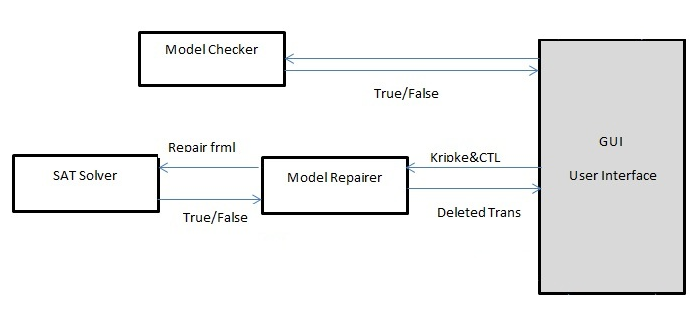
\includegraphics[width=15cm,height=13cm,keepaspectratio]{modules}
\caption{Tool main modules}
\label{fig4:Modules}
\end{figure}




\section{Experimental Results}

\begin{table}[th]
\centering
\begin{tabular}{c|c|cl}
 \# Processes     & Old Tool        & Our Tool    \\ \hline  
2                   & 93                  & 107             \\
3                   & 1,210                   & 104              \\
4                   & Out of memory    & 248            
\end{tabular}
\caption{Times (in Miliseconds) taken to repair mutual exclusion \wrt safety, single kripke strcuture}
\label{table:benchMutex}
\end{table}

\begin{table}[th]
\centering
\begin{tabular}{c|c|cl}
 \# Processes     & Old Tool        & Our Tool   \\  \hline  
2                   & 67                  & 63             \\
3                   & 460                   & 107              \\
4                   & 1,105      & 164            
\end{tabular}
\caption{Times (in Miliseconds) taken to repair barrier  \wrt synchronisation, single kripke structure}
\label{table:benchBarrier}
\end{table}



\section{Technical Details}

\subsection{Algorithm for Generating the Repair Formula}
The Algorithm is provided in pseudo code in the appendix on the last page.
\clearpage
\subsection{Constructing The Synchronisation Formula}
\begin{lstlisting}
/**
 * Construct the structure formula, the formula that synchronizes transitions
 * for each processes over all the structures.
 * 
 * <p>The formula necessitates that for a specific process, if all the transitions
 * taking that process from one state to another were deleted in one Structure, they 
 * must be also deleted in all of the structures.</p>
 * 
 * @return the Structure Formula for this MultiKripkeStructure.
 */
protected AbstractExpression getSynchFormula() {
	HashMap<String, EquivalenceOperator> equiMap = new HashMap<String, EquivalenceOperator>();
	Integer[] allProcesses = getParticipatingProcesses();
	AndOperator andOp = new AndOperator();
	for(int p : allProcesses) {
		ArrayList<KripkeStructure> structures = new ArrayList<KripkeStructure>();
		ArrayList<Integer> indices = new ArrayList<Integer>();
		for(int i = 0; i < processes.size(); i++) {
			int[] pairs = processes.get(i);
			if(pairs[0] == p || pairs[1] == p) {
				structures.add(kripkeList.get(i));
				indices.add(pairs[0] == p ? 0 : 1);
			}
		}
		
		for(int i = 0; i < structures.size(); i++) {
			KripkeStructure s = structures.get(i);
			HashMap<String, ArrayList<KripkeTransition>> map = s.mapLabelToTransition(indices.get(i));
			
			for(String key : map.keySet()) {
				if(equiMap.get(key) == null)
					equiMap.put(key, new EquivalenceOperator());
				
				OrOperator orOp = new OrOperator();
				for(KripkeTransition t : map.get(key)) {
					orOp.or(new BooleanVariable(t.getVarName()));
				}
				
				equiMap.get(key).equate(orOp);
			}
		}
	}
	
	for(String key : equiMap.keySet()) {
		andOp.and(equiMap.get(key));
	}
	
	return andOp;
}
\end{lstlisting}

\subsection{UML Diagram for CTL Logic API}

\begin{figure}[H]
\centering
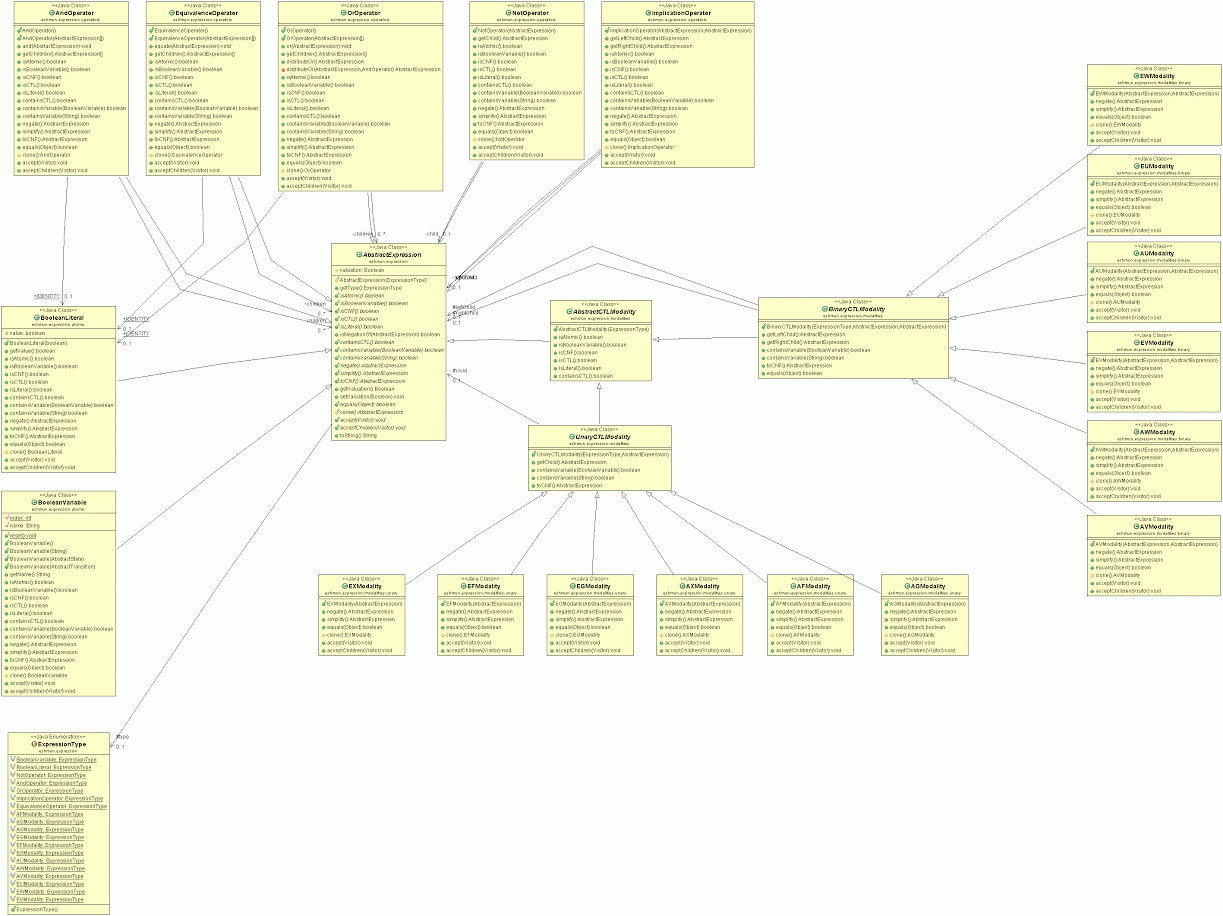
\includegraphics[width=15cm,height=13cm,keepaspectratio]{logic.jpg}
\caption{Tool main modules}
\label{fig4:Modules}
\end{figure}


\subsection{UML Diagram for the Models Data Structures}

\begin{figure}[H]
\centering
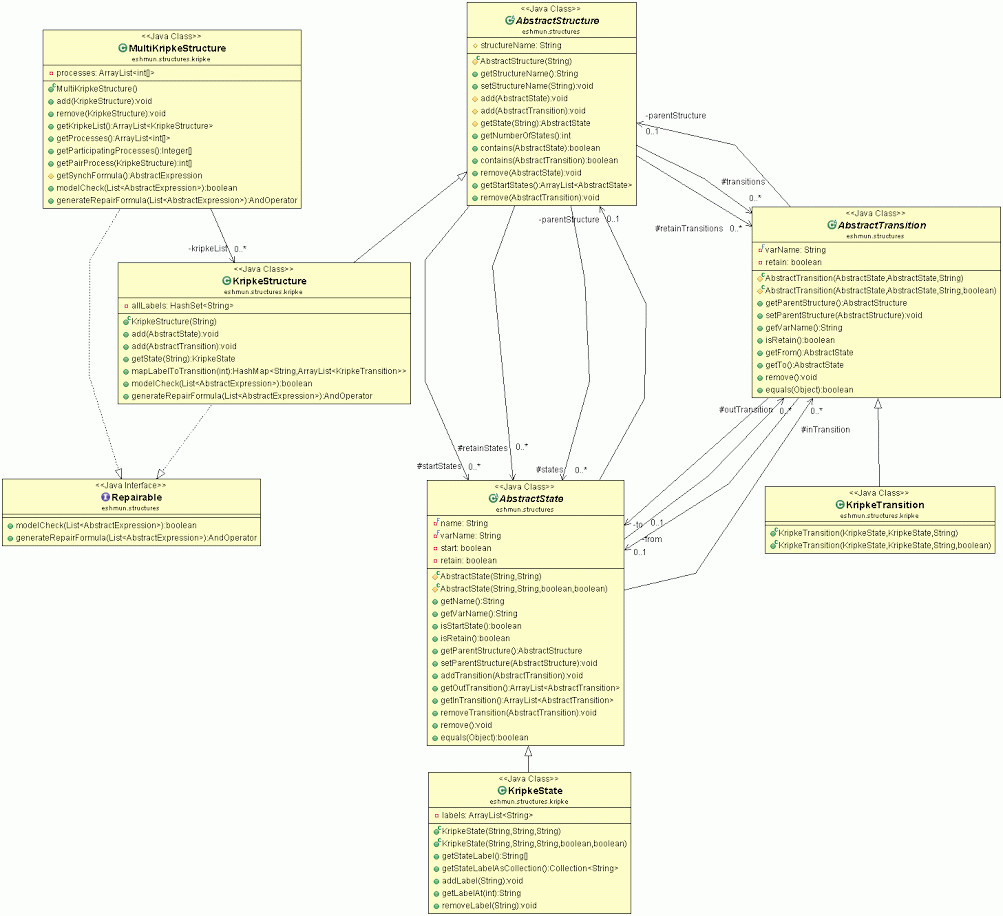
\includegraphics[width=15cm,height=13cm,keepaspectratio]{structures.jpg}
\caption{Tool main modules}
\label{fig4:Modules}
\end{figure}



\begin{figure}[th]
  \centering
  \framebox{
    \begin{minipage}{1.0\linewidth}
    \begin{tabbing}
    mmm\=mmm\=mmm\=mmm\=mmm\=mmm\=mmm\=mmm\=mmm \kill
       \>\ul{\propagateA{$s,\xi$}}\\[1ex]

       \>\IF $\xi \in \old{s}$ \THEN \`\cmnt $\xi$ has already been processed\\
       \>   \>$\setDel{\new{s}}{\xi}$; \RETURN\\

       \> \cmnt already checked for larger index\\
       \>\IF $\xi = \A[\vphi \V \psi]^m$ and $\A[\vphi \V \psi]^{m'} \in \old{s}$ for some $m' \ge m$ \THEN \\
       \>   \>$\setDel{\new{s}}{\xi}$; \RETURN\\

       \>\cmnt already checked for larger index\\  %CHECK IF THIS IS CORRECT FOR NEGATED CASE
       \>\IF $\xi = \E[\vphi \V \psi]^m$ and $\E[\vphi \V \psi]^{m'} \in \old{s}$ for some $m' \ge m$ \THEN \\
       \>   \>$\new{s} := \new{s} - \xi$; \RETURN\\[1ex]



       \>\CASE $\xi$:  \`\cmnt $\xi$ has not been processed \\%[1ex]

       \>   \>$\xi = \neg \vphi$: \\
       \>   \>   \>$\setInsS{\new{s}}{\vphi}$;
                         $\conjoinA{\mstr{X_{s,\neg\vphi} \equiv \neg X_{s,\vphi}}}$;\\

       \>   \>$\xi = \vphi \lor \psi$: \\
       \>   \>   \>$\setInsS{\new{s}}{\vphi,\psi}$;
                         $\conjoinA{\mstr{X_{s,\vphi \lor \psi} \equiv X_{s,\vphi} \lor X_{s,\psi}}}$;\\

       \>   \>$\xi = \vphi \land \psi$: \\
       \>   \>   \>$\setInsS{\new{s}}{\vphi,\psi}$;
                         $\conjoinA{\mstr{X_{s,\vphi\land\psi} \equiv X_{s,\vphi} \land X_{s,\psi}}}$;\\

       \>   \>$\xi = \AX \vphi$: \\
       \>   \>   \>\FORALL $t \in R[s]: \setInsS{\new{t}}{\vphi}$ \ENDFOR;\\
       \>   \>   \>$\conjoinA{\mstr{\AND_{t \in R[s]} (E_{s,t} \imp X_{t,\vphi})}}$\\

       \>   \>$\xi = \EX \vphi$: \\
       \>   \>   \>\FORALL $t \in R[s]: \setInsS{\new{t}}{\vphi}$ \ENDFOR;\\
       \>   \>   \>$\conjoinA{\mstr{\OR_{t \in R[s]} (E_{s,t} \land X_{t,\vphi})}}$\\


       \>   \>$\xi = \A[\vphi \V \psi]$: \\
       \>   \>   \>$\setInsS{\new{s}}{\A[\vphi \V \psi]^n}$;\\
       \>   \>   \>$\conjoinA{\mstr{X_{s,\A[\vphi \V \psi]} \equiv X^n_{s,\A[\vphi \V \psi]}}}$;\\

       \>   \>$\xi = \A[\vphi \V \psi]^m$, $m \in \oneton$: \\
       \>   \>   \>$\setInsS{\new{s}}{\vphi,\psi}$;\\
       \>   \>   \>\FORALL $t \in R[s]: \setInsS{\new{t}}{\A[\vphi \V \psi]^{m-1}}$;\\
       \>   \>   \>$\conjoinA{\mstr{X_{s,\A[\vphi \V \psi]}^m \equiv 
                       X_{s,\psi} \land 
                             (X_{s,\vphi}
                              \lor 
                             \AND_{t \in R[s]} (E_{s,t} \imp X_{t,\A[\vphi \V \psi]}^{m-1}))}}$\\

       \>   \>$\xi = \A[\vphi \V \psi]^0$: \\
       \>   \>   \>$\setInsS{\new{s}}{\psi}$;\\
       \>   \>   \>$\conjoinA{\mstr{X_{s,\A[\vphi \V \psi]}^{0} \equiv X_{s,\psi}}}$\\


       \>   \>$\xi = \E[\vphi \V \psi]$: \\
       \>   \>   \>$\setInsS{\new{s}}{\E[\vphi \V \psi]^n}$;\\
       \>   \>   \>$\conjoinA{\mstr{X_{s,\E[\vphi \V \psi]} \equiv X^n_{s,\E[\vphi \V \psi]}}}$;\\

       \>   \>$\xi = \E[\vphi \V \psi]^m$, $m \in \oneton$: \\
       \>   \>   \>$\setInsS{\new{s}}{\vphi,\psi}$;\\
       \>   \>   \>\FORALL $t \in R[s]: \setInsS{\new{t}}{\A[\vphi \V \psi]^{m-1}}$;\\
       \>   \>   \>$\conjoinA{\mstr{X_{s,\E[\vphi \V \psi]}^m \equiv 
                       X_{s,\psi} \land 
                             (X_{s,\vphi}
                              \lor 
                             \OR_{t \in R[s]} (E_{s,t} \land X_{t,\E[\vphi \V \psi]}^{m-1}))}}$\\

       \>   \>$\xi = \E[\vphi \V \psi]^0$: \\
       \>   \>   \>$\setInsS{\new{s}}{\psi}$;\\
       \>   \>   \>$\conjoinA{\mstr{X_{s,\E[\vphi \V \psi]}^{0} \equiv X_{s,\psi}}}$\\


       \>\ENDCASE;\\

%       \>$\marked(s,\xi) \gt \true$\\
       \>$\setDelS{\new{s}}{\xi}$; \`\cmnt remove $\xi$ from $\mathit{new}$ since it has been processed\\
       \>$\setInsS{\old{s}}{\xi}$; \`\cmnt record that $\xi$ has been processed\\\\


    \end{tabbing}
    \end{minipage}
}
  \caption{Formula propagation.}
  \label{fig:propagate}
\end{figure}


\section{Future Work}

\begin{itemize}
  \item Support more formal models for concurrent programs: I/O Automata, BIP.
  \item Extend logic to include ATL(Alternating Temporal Logic), which is more expressive.
  \item Develop an additive model repair algorithm that allows repair to be carried out by adding new states or transitions.
\end{itemize}

\end{document}

